\chapter{\IfLanguageName{dutch}{Resultaten}{Results}}
\label{ch:res}

In dit onderdeel zal de accuraatheid en de efficiëntie van het ontwikkelde proof of concept (POC) worden getest. Ook zal hier worden bekeken hoeveel utterances er bij de 'Review endpoint' utterances komen met en zonder de implementatie van de proof of concept.

Eerst en vooral zullen er per intent een 6-tal voorbeeld-utterances worden opgesteld. Dat zal gedaan worden voor de volgende intents: AddMore, ClearBasket, DeleteItem, FindItem, Greeting, Help, RemoveMove, ShowBasket, ShowProfile, Stop en UpdateProfile. Aan de hand van deze voorbeelden zal er getest worden.

Deze testen zullen verschillende keren worden uitgevoerd. Er zijn een aantal parameters in de POC die kunnen worden aangepast. Uit deze testen zullen uiteindelijk blijken wat de beste parameters zijn voor de optimale accuraatheid.

\section{Testdata}
\label{sec:testdata}

De testdata van deze opzet bevindt zich in bijlage. De eerste 4 voorbeeld-utterances van elke intent zullen als input doorgestuurd worden naar de bot, dus naar LUIS zelf. Dit zal gedaan worden met en zonder het uitgewerkte proof of concept. Dan zal er gekeken worden hoeveel van deze utterances er bij 'Review endpoint' komen wanneer er wordt gewerkt op de gewone manier zonder het uitgewerkte POC en daarna zal gekeken worden hoeveel er bijkomen als er wordt gewerkt met het gemaakte POC. De laatste 2 voorbeeld-utterances van elke intent zullen gebruikt worden om te controleren hoe hard de accuraatheid per utterance is veranderd vóór en na het ingeven van de 4 eerste voorbeeld-utterances. Dit zal ook gedaan worden eerst op de gewone manier en dan met het POC.

\section{Uitwerking}
\label{sec:uitwerking}

Na het opzetten van de testdata kan er uiteindelijk getest worden. Op de site van LUIS zelf is er een tool ter beschikking om meerdere utterances uit te voeren en daar de resultaten kan bekijken, genaamd 'batch testing'. De bedoeling is dat alle inputs die getest moeten worden in een json-formaat moeten worden geüpload. In deze json dient bij elke input de intent meegegeven te worden en eventueel de entities. De entities zijn hier niet noodzakelijk omdat LUIS deze er automatisch uithaalt. Eenmaal de json is opgesteld, kan deze worden geïmporteerd in de 'batch testing panel'. LUIS leest deze json dan in en als ze verwerkt is, kan de test worden uitgevoerd.

Aan de hand van hoe groot de test is, zal deze redelijk snel worden uitgevoerd en kan er al direct naar de resultaten worden gekeken. Hier kan er gezien worden hoeveel van de utterances geslaagd zijn en kan er per utterance dan nog eens in detail bekeken worden met een percentage aan welke intent deze wordt gelinkt.

Bij de testen die zullen uitgevoerd worden, zal er telkens dezelfde set aan input gebruikt worden. Dit is een test die éénmaal zal worden uitgevoerd vóór al de andere testen beginnen en éénmaal na alle andere testen. Aan de hand van deze test zal er bekeken worden in welke mate de POC invloed heeft op de scores die LUIS geeft aan elke utterance samen met de intent. Idealiter zou zijn dat de scores stijgen. Als deze zouden dalen, zou dat betekenen dat er utterances gelinkt zijn aan de verkeerde intent. Dit is iets dat zeker moet worden vermeden.

Bij het uitvoeren van deze test zijn er 22 inputs die getest worden. Hier is gebleken dat LUIS 2 van die 22 utterances aan de foute intent heeft gelinkt. Dit kan komen door de beperkte aantal voorbeeld-utterances die LUIS bevat. Het zou pas een probleem zijn moest uit de laatste test blijken dat dit aantal zou stijgen.

Nu dat deze test heeft gelopen, kan er aan de slag worden gegaan met de andere testdata, de 4 andere voorbeeld-inputs per intent, in totaal zijn dit 44 inputs. Deze voorbeeldzinnen zullen via de 'Bot Framework Emulator' worden ingegeven, zo zullen de zinnen ook binnenkomen in LUIS als er echte gebruikers met de bot zouden praten via messenger bijvoorbeeld.

Omdat dit 44 zinnen zijn en dit is vrij veel om deze meerdere keren handmatig te moeten ingeven, zal er een manier moeten gezocht worden om dit te automatiseren. De oplossing die hiervoor is gevonden, is met een programma genaamd 'MurGaa auto talker'. In dit programma kunnen al de inputs éénmaal worden ingegeven en dient er verder niets meer gedaan te worden met deze. Er kan ingesteld worden dat dit programma de berichten verstuurd naar de emulator. Elke 5 seconden wordt er zo automatisch een bericht gestuurd naar de chatbot tot als alle inputs zijn ingegeven. Op deze manier dient niet elke zin apart te worden ingegeven en zal dit veel tijd besparen.

Al deze 44 inputs worden nu automatisch ingegeven in de emulator. Deze emulator stuurt deze dan naar de POC die dan LUIS zal aanroepen. Er zullen hier ook 2 testen worden uitgevoerd. Bij de eerste test zal de POC de utterances gewoon doorsturen naar LUIS zonder verder iets te doen, zoals het altijd al gebeurde dus. Bij de tweede test zal het systeem worden aangezet die is ontwikkeld voor het controleren van elke utterance en deze dan zal toevoegen aan LUIS indien dat kan.

Door hier op deze 2 manieren te testen zal er in LUIS worden gekeken na elke test hoeveel van deze 44 inputs er komen in de 'Review endpoint utterances' tab en zal zo berekend kunnen worden hoeveel percent minder utterances in deze tab komen als het systeem is ingeschakeld.

Na het doorlopen van de eerste test is gebleken dat zo goed als alle inputs komen bij 'Review endpoint utterances' wat dus zeer inefficiënt is. Hier is er dus zeer veel werk nodig om elke utterance te bekijken en deze te valideren. Na de eerste test is het systeem ingeschakeld en zal een tweede test worden uitgevoerd. De 'MurGaa auto talker' zal weer de 44 inputs doorsturen naar de emulator. Uit de tweede test is gebleken dat in plaats van 40 utterances die komen bij 'Review endpoint utterances' er nu maar 20 meer inkomen. Dit betekent dat 55 percent van de utterances niet meer bekeken zal worden want deze zijn al automatisch gelinkt aan de juiste intent. Na het controleren of deze wel effectief correct zijn toegevoegd, zijn er geen fouten gevonden. Het kan wel zijn dat LUIS soms een entity niet vindt of fout benoemt. Dit komt door het beperkt aantal utterances per intent.

Nu dit allemaal is getest en de resultaten positief zijn, kan nu de tweede batchtest worden gedaan. LUIS is nu veranderd doordat de POC automatisch nieuwe utterances heeft toegevoegd een de intent. Hier kan er dan gezien worden of dit wel effectief niet is verslechterd en eventueel beter is geworden.

\begin{figure}[h!]
	\centering
	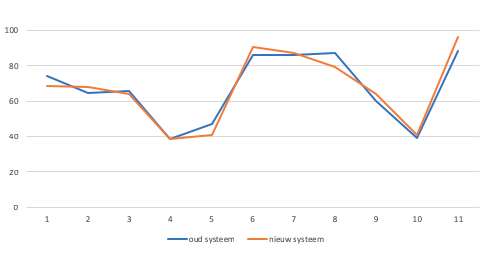
\includegraphics[height=8cm]{img/grafiek.png}
	\caption{Resultaat batch testen}
	\label{fig:batchtest}
\end{figure}

In afbeelding \ref{fig:batchtest} is er duidelijk te zien dat door de implementatie van het nieuwe systeem geen verbetering maar ook geen verslechtering is van LUIS. De x-as stelt de utterances voor en de y-as het percantage van zekerheid. Bij sommige van de 11 utterances hier is het resultaat een beetje beter en dat is wat we wouden zien. Bij een aantal utterances is er ook een lichte verslechtering te zien. Dit komt doordat er per intent een beperkt aantal utterances zijn voorzien en deze utterances lagen allemaal zeer dicht bij elkaar, met andere woorden was de woordkeuze niet zo verschillend. In de testdata is er al meer gewerkt met echte zinnen en andere woordkeuzes. Door deze nieuwe utterances zullen de utterances per intent meer uiteenliggen met het gevolg dat de utterances van één bepaalde intent dichter zullen liggen bij de utterances van een andere intent. Bijvoorbeeld 'Can you please show my basket' en 'Can you please show my profile' liggen veel dichter bij elkaar dan 'show my basket' en 'what's my name'.

Er kan hier ook worden gekeken om een aantal parameters aan te passen om te kijken of dit de resultaten zou beïnvloeden. Hoe de resultaten hier beschreven zijn is met parameters die goed geschikt zijn voor deze LUIS-testset. Elke utterance kwam bij de juiste intent terecht en de resultaten van de batchtest waren zelf lichtjes beter dan ervoor. Er kan altijd nog wel wat lichtjes met gespeeld worden met deze parameters maar er moet ook rekening gehouden worden met nieuwe utterances die er eventueel aan kunnen worden toegevoegd. Een beetje speling houden kan altijd voordelig uitkomen.

%parameter

%2 zinnen niet herkent
